\documentclass[12pt]{article}
\usepackage[utf8]{inputenc}
\usepackage[margin=1in]{geometry}
\usepackage[spanish]{babel}\decimalpoint
\usepackage{setspace}\onehalfspacing
\usepackage{parskip} % Espacio entre parrafos.
\usepackage{graphicx} % Para usar comando \includegraphics[]{}
\usepackage{amssymb} % Para usar el simbolo del conj. de los Reales.
\usepackage{amsmath} % Para usar columnas vectoriales.
\usepackage{multirow} % Para unir multiples filas en una tabla.
\usepackage{hyperref} % Siempre debe ser el ultimo paquete.


\setcounter{tocdepth}{2} % Que no incluya subsubsections en la tabla de contenidos (toc).

%================================

\title{Clase 20: Teorema Fundamental del Cálculo (Parte 2).}
\author{MIT 18.01: Single Variable Calculus.}
\date{}

\begin{document}

\maketitle

\begin{abstract}
\noindent Continuando con el vínculo entre las integrales definida e indefinida, estudiaremos la \textbf{segunda parte del Teorema Fundamental del Cálculo} (TFC 2). Primero, haremos una comparación entre el TFC 1 y el Teorema del Valor Medio, la cual nos dará información relevante para, en segundo lugar, estudiar el TFC 2 y demostrar ambas partes de este teorema fundamental.
\end{abstract}

\section{Comparando el TVM con el TFC 1.}

La clase pasada, usando el TFC 1, evaluamos integrales definidas a partir de sus antiderivadas. Ahora lo haremos al revés, tomando el integrando para evaluar su antiderivada y lo ilustraremos, primero, comparando el Teorema del Valor Medio (TVM) con el TFC 1.

Recordemos que el TVM señala que si una función $f(x)$ es continua en $[a, \ b]$ y derivable en $(a, \ b)$, podemos garantizar que:
\[
  \frac{f(b) - f(a)}{b - a} = f'(c) \qquad \forall c \in (a, \ b)
\]
Por otra parte, el TFC 1 indica que si $f(x)$ es continua en $[a, \ b]$ y si se cumple que $F'(x) = f(x)$, entonces:
\[
  \int_{a}^{b} f(x)dx = F(b) - F(a)
\]
Ahora, establezcamos que $\Delta F = F(b) - F(a)$, que $\Delta x = b - a$. Esto implica que:
\[
  \Delta F = \int_{a}^{b} f(x)dx
\]
Luego, dividamos la igualdad de arriba por $\Delta x = b - a$.

\[
  \frac{\Delta F}{\Delta x} = \frac{1}{\Delta x} \cdot \int_{a}^{b} f(x)dx
\]
El lado derecho de esta ecuación es el \textbf{valor promedio} (\textit{average}) de $f(x)$ o $F'(x)$ y que denotaremos como PROM$(F'(x))$.
\[
  \frac{\Delta F}{\Delta x} = \text{PROM}(F'(x))
\]
En otras palabras, el cambio en $F(x)$ es igual al valor promedio de $f(x) = F'(x)$.

Para volver al TFC 1, multipliquemos esta ecuación por $\Delta x$.
\[
  \Delta F = \text{PROM}(F'(x)) \cdot \Delta x
\]
Ahora, escribamos el TVM usando a $F(x)$.
\[
  \frac{F(b) - F(a)}{b - a} = F'(c) \qquad \forall c \in (a, \ b)
\]
Lo cual es lo mismo que:
\[
  \frac{\Delta F}{\Delta x} = F'(c) \qquad \forall c \in (a, \ b)
\]
Y si multiplicamos esta ecuación por $\Delta x$, entonces
\[
  \Delta F = F'(c) \cdot \Delta x
\]
La similitud que existe entre el TFC 1 y el TVM, es que ambos son valores que podemos asegurar que están entre los valores máximos y mínimos de $F'(x)$ multiplicados por $\Delta x$.
\begin{align*}
\text{TFC 1} &\longrightarrow
\min_{a < x < b}(F'(x)) \cdot \Delta x \leq
\text{PROM}(F'(x)) \cdot \Delta x \leq
\max_{a < x < b}(F'(x)) \cdot \Delta x
\\
\text{TVM} &\longrightarrow
\min_{a < x < b}(F'(x)) \cdot \Delta x \leq
F'(c) \cdot \Delta x \leq
\max_{a < x < b}(F'(x)) \cdot \Delta x
\end{align*}
Pero el TFC 1 podemos conocerlo, es un valor exacto y está entre los valores máximo y mínimo  de $F'(x)$ multiplicados por $\Delta x$. Ésto no es posible con el TVM, porque solo tenemos garantía de que existe $F'(c)$, pero no qué valor es en particular.

Es por ello que si conocemos la integral, es mejor encontrar el cambio en $F(x)$ a partir del TFC 1 en vez del TVM, por la vaguedad de este último.

\newpage

\textbf{Ejemplo 1.} \quad Sean $F'(x) = 1/(1 + x)$ y $F(0) = 1$. ¿Para qué valores $A$ y $B$ se cumple que $A < F(4) < B$? Búsquelos a partir (1) del TVM y (2) del TFC 1.

\textbf{Solución.} \quad Comencemos escribiendo el (1) TVM de la siguiente manera:
\[
  \frac{F(4) - F(0)}{4 - 0} = \frac{1}{1 + c} \quad \forall c \in (0, \ 4)
\]
Y despejemos $F(4) - F(0)$, multiplicando la ecuación por $4$.
\[
  F(4) - F(0) = \frac{1}{1 + c} \cdot 4
\]
No conocemos $x = c$, pero sabemos que se encuentra entre $0$ y $4$. Eso significa que:
\begin{align*}
F(4) - F(0) &= \frac{1}{1 + 0} \cdot 4 & F(4) - F(0) &= \frac{1}{1 + 4} \cdot 4 \\
            &= 4                       &             &= \frac{4}{5}
\end{align*}
Por lo tanto, podemos asegurar que:
\[
  \frac{4}{5} \leq F(4) - F(0) \leq 4
\]
Queremos saber entre qué valores está $F(4)$ y como $F(0) = 1$, sumemos por $1$ a la desigualdad.
\[
  A = \frac{9}{5} \leq F(4) \leq 5 = B
\]
Ahora veámoslo con el (2) TFC 1 y mantengamos la diferencia $F(4) - F(0)$.
\[
  F(4) - F(0) = \int_{0}^{4} \frac{1}{1 + x} dx
\]
El valor más alto que puede tomar el integrando es $0$ y el más bajo es $4$. Es decir:
\begin{align*}
\int_{0}^{4} \frac{1}{1 + 4} dx &< \int_{0}^{4} \frac{1}{1 + x} dx < \int_{0}^{4} \frac{1}{1 + 0} dx \\
\int_{0}^{4} \frac{1}{5} dx &< \int_{0}^{4} \frac{1}{1 + x} dx < \int_{0}^{4} 1 dx \\
4 \cdot \frac{1}{5} &< F(4) - F(0) < 4 \cdot 1 \\
\frac{4}{5} &< F(4) - F(0) < 4
\end{align*}
Las desigualdades son estrictas porque los valores de las esquinas izquierda y derecha son áreas de rectángulos. En otras palabras, lo que estamos haciendo es estimar el valor de $F(4) - F(0)$ por medio de dos \textbf{sumas de Riemann}: una \textbf{inferior} (igual a $4/5$) y otra \textbf{superior} (igual a $4$), con una división (un rectángulo) para cada caso.

\begin{figure}[hbt!]
\centering
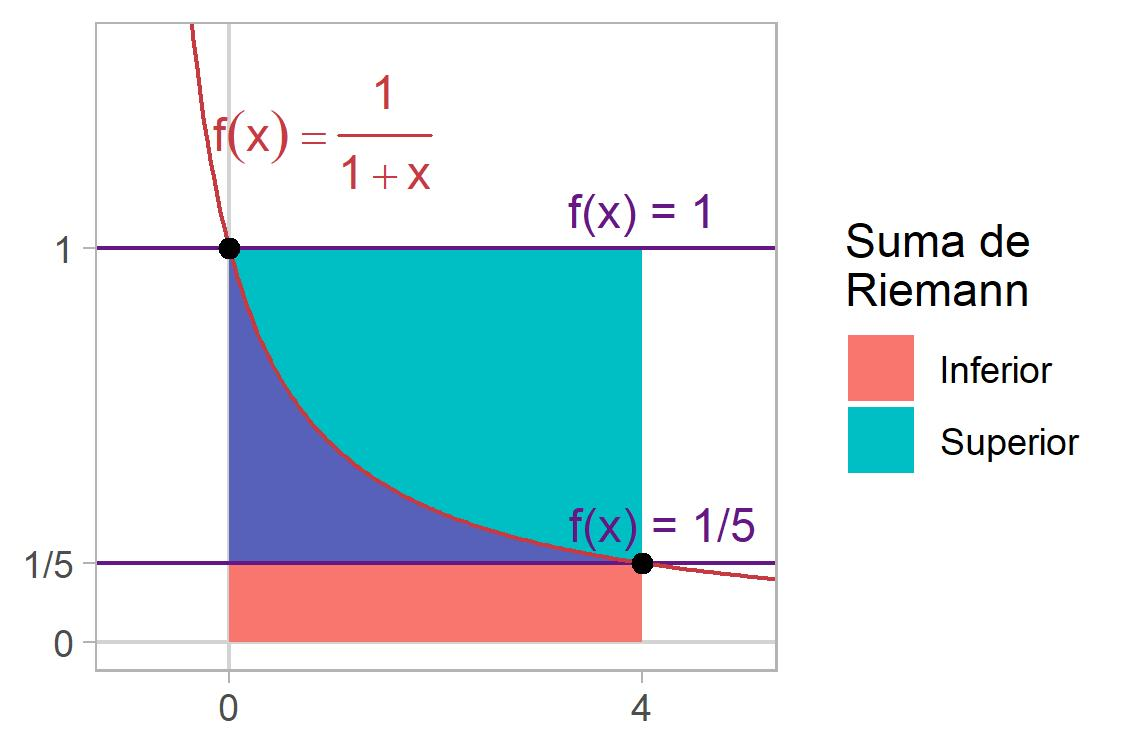
\includegraphics[scale=0.7]{img/tvm_tfc1_example.jpg}
\end{figure}

Finalmente, debido a que $F(0) = 1$, sumamos por ese valor a la desigualdad.
\[
  \frac{9}{5} < F(4) < 5
\]
En ese sentido, es más fácil conocer el valor de $F(4)$ usando el TFC 1, porque solo basta con dividir infinitamente el área $\int_{0}^{4} 1/(1 + x)dx$. En cambio, con el TVM aquello nunca lo sabremos explícitamente. Es por ello que, al tener la integral, optamos por el primer teorema, sin que el segundo deje de ser relevante (lo veremos más adelante).

\section{Teorema Fundamental del Cálculo (TFC 2).}

La otra manera en que evaluaremos el integrando por medio de su antiderivada, es a partir de la \textbf{segunda parte del Teorema Fundamental del Cálculo} (TFC 2), que indica lo siguiente:

\textbf{Teorema.} \quad Si $f(x)$ es una función continua y
\[
  G(x) = \int_{a}^{x} f(t)dt \qquad (\text{donde } a \leq t \leq x)
\]
entonces:
\[
  \frac{d}{dx}G(x) = f(x)
\]
Lo que nos dice el TFC 2 es que si se cumplen sus dos hipótesis, podemos confirmar que $f(x)$ es una tasa de cambio instantánea o el integrando de la integral que definimos en $G(x)$. En otras palabras, evaluamos al integrando a partir de su antiderivada.

Por otra parte, debemos tener en consideración que:

\begin{enumerate}
\item $a$ se mantiene fija, mientras que $x$ varía.
\item $t$ es una variable ficticia (\textit{dummy variable}).
\end{enumerate}

Se denota a la variable ficticia $t$ en la integral porque solo es útil cuando a $x$ lo mantenemos fijo\footnote{Ahí podemos evaluar la integral por medio del TFC 1.}. En ese caso, los límites de la integral son $t = a$ y $t = x$. Por lo tanto, nos sirve para diferenciarla de $a$ y $x$ cuando aplicamos el TFC 2, ya que ahí no es de nuestro interés.

Una de las relevancias del TFC 2, es que con él podemos garantizar que $G(x)$ resuelve la ecuación diferencial:
\[
  \frac{d}{dx}y = f(x) \quad \text{para la condición inicial } y(a) = 0
\]
Se especifica la condición inicial, porque la integral definida en el intervalo $[a, \ a]$ es igual a cero.

\textbf{Ejemplo 2.} \quad Calcule $\frac{d}{dx} \left(\int_{1}^{x} (1/t^{2})dt\right)$.

\textbf{Solución.} \quad Acá solo debemos aplicar el TFC 2. En primer lugar, veamos que:
\[
  G(x) = \int_{1}^{x} \frac{1}{t^{2}} dt
\]
Y como $1/t^{2}$ es continua para $t \neq 0$, por el TFC 2 obtenemos que:
\[
  \frac{d}{dx} G(x) = \frac{d}{dx} \left(\int_{1}^{x} \frac{1}{t^{2}} dt\right) = \frac{1}{x^{2}}
\]
Para corroborarlo (no siempre es necesario), podemos hacerlo a partir de la integral y usando el TFC 1.
\[
  G(x) = \int_{t = 1}^{t = x} \frac{1}{t^{2}} dt
       = \left.\frac{t^{-1}}{-1}\right|_{1}^{x}
       = \left. -\frac{1}{t}\right|_{1}^{x}
       = - \frac{1}{x} + 1
\]
Y, luego, calculamos $G'(x)$ que debe ser igual a $1/x^{2}$, en caso contrario está errado.
\[
  \frac{d}{dx} G(x) = \frac{d}{dx} \left(-\frac{1}{x} + 1\right) = \frac{1}{x^{2}}
\]

\subsection{Demostración TFC 2.}

La demostración del TFC 2 podemos hacerlo de forma geométrica.

Sea $y = f(x)$ una función continua y $G(x)$ el área bajo su curva en el intervalo $[a, \ x]$. Como $x$ varía, digamos que incrementa en $x + \Delta x$, haciendo que este área aumente y cuyo cambio lo denotamos como $\Delta G$.

\begin{figure}[hbt!]
\centering
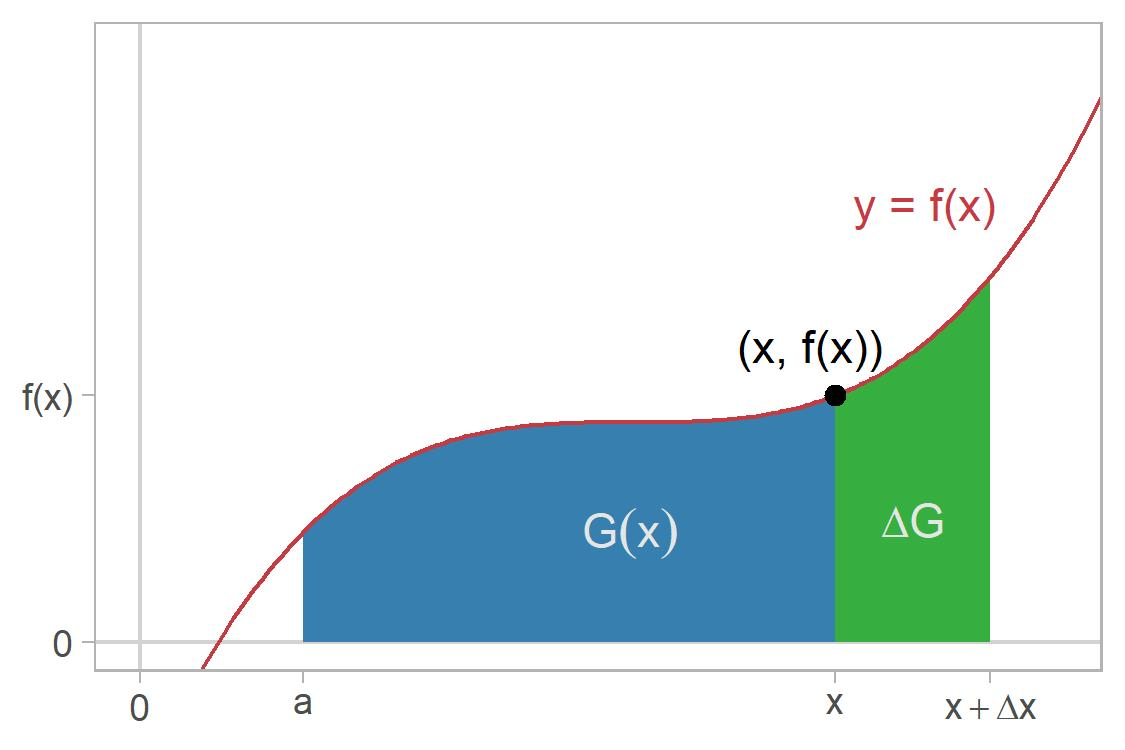
\includegraphics[scale=0.7]{img/ftc2_proof.jpg}
\end{figure}

Para conocer el área $\Delta G$, podemos aproximarnos a él dividiéndolo en rectángulos donde el primero toca a la curva en $(x, \ f(x))$. En ese sentido, podemos decir que:
\[
  \Delta G \approx \Delta x \cdot f(x)
\]
Y si dividimos por $\Delta x$, entonces:
\[
  \frac{\Delta G}{\Delta x} \approx f(x)
\]
Esta aproximación se irá haciendo más precisa a medida que $\Delta x \to 0$. Es decir:
\[
  \lim_{\Delta x \to 0} \frac{\Delta G}{\Delta x} = f(x)
\]
donde esta igualdad se cumple debido a que $f(x)$ es continua.

Además, por la definición de la derivada, el lado izquierdo de la ecuación de arriba corresponde a $G'(x)$.
\[
  \lim_{\Delta x \to 0} \frac{\Delta G}{\Delta x} = G'(x)
\]
En consecuencia:
\[
  G'(x) = f(x) \quad (\text{Q.E.D})
\]

\subsection{Demostración TFC 1.}

En este caso, también establezcamos que $f(x)$ es una función continua y que $F'(x) = f(x)$. Además, digamos que $G(x) = \int_{a}^{x} f(t)dt$, donde $x$ varía, $a$ es constante y $t$ es una variable ficticia.

Anteriormente vimos que la conclusión del TFC 2 señala que $G'(x) = f(x)$. Por tanto es válido establecer que:
\[
  F'(x) = G'(x)
\]
Si igualamos esta ecuación por cero y aplicamos propiedades de las derivadas, entonces:
\[
  F'(x) - G'(x) = (F(x) - G(x))' = 0
\]
Recordemos que una de las conclusiones del TVM es que si una derivada es igual a cero en un punto de una función, significa que ahí esta última es constante:
\[
  F(x) - G(x) = C \quad (C \text{ es constante})
\]
Al despejar $F(x)$:
\[
  F(x) = G(x) + C
\]
El TFC 1 señala que:
\[
  \int_{a}^{b} f(x)dx = F(b) - F(a)
\]
Y como $F(x) = G(x) + C$:
\[
  \int_{a}^{b} f(x)dx = (G(b) + C) - (G(a) + C) = G(b) - G(a)
\]
Finalmente, al inicio señalamos que $G(x) = \int_{a}^{x} f(t)dt$. En consecuencia:
\[
  \int_{a}^{b} f(x)dx = G(b) - G(a)
                      = \int_{a}^{b} f(x)dx - \int_{a}^{a} f(x)dx
                      = \int_{a}^{b} f(x)dx - 0
                      = \int_{a}^{b} f(x)dx
\]
Q.E.D.

En el Ejemplo 2, vimos por el TFC 2 que:
\[
  G(x) = \int_{1}^{x} \frac{1}{t^{2}} dt \qquad G'(x) = \frac{1}{x^{2}} = f(x)
\]
Por otra parte, como $f(x) = G'(x)$, a partir del TFC 1 obtuvimos que:
\[
  G(x) = \int_{1}^{x} \frac{1}{t^{2}} dt = 1 - \frac{1}{x}
\]
Lo interesante es que en la integral definida que vemos a continuación, se cumple la siguiente igualdad:
\[
  \int_{1}^{2} \frac{1}{t^{2}} = \left.-\frac{1}{t}\right|_{1}^{2}
                               = \left.\left(1 - \frac{1}{t}\right)\right|_{1}^{2}
\]

\subsection{Buscando ``nuevas'' funciones.}

El TFC 2 es de gran ayuda para encontrar soluciones a ecuaciones diferenciales.

\textbf{Ejemplo 3.} \quad Busque la solución de $L'(x) = 1/x$ cuya condición inicial es $L(1) = 0$.

\textbf{Solución.} \quad Cuando estudiamos ecuaciones diferenciales, vimos solo el método de separación de variables para resolverlas, pero no es posible aplicarlo a todos los casos y este ejemplo es uno de ellos. No obstante, a partir del TFC 2 sí podemos hacerlo, obteniendo la siguiente solución para $L(1) = 0$.
\[
  L(x) = \int_{1}^{x} \frac{1}{t} dt
\]
Establecimos el límite inferior de esta integral igual a uno, porque es necesario para que $L(1) = 0$:
\[
  L(1) = \int_{1}^{1} \frac{1}{t} dt = 0
\]
Algo interesante de este ejemplo, es que $L(x)$ corresponde a $\ln(x)$, pero no es escrita como tal. En general, las funciones que se encuentran a partir del TFC 2 se dice que son \textbf{totalmente} ``\textbf{nuevas}'' porque no pueden ser expresadas en términos de otras conocidas, como la función $e^{x}$, las trigonométricas, etc.

Ahora, escribimos funciones ``nuevas'', porque en algunos casos se comportan como otras existentes, como es en el caso de este ejemplo, pero nunca podremos escribirlas de esa manera.

No obstante, el caso del $\ln(x)$ proviene justamente en la forma de $L(x)$. En otras palabras, solo puede ser obtenida desde el Cálculo y es por ello que se la categoriza como una \textbf{función trascendental} porque solo existe desde esta área de la matemática y está fuera del alcance del álgebra\footnote{También ocurre con algunos números, como es el caso de $\pi$.}.

\end{document}
